\documentclass[conference,a4paper]{IEEEtran}
\usepackage{amsmath}
\usepackage{graphicx}
\usepackage{stfloats}
\usepackage{booktabs}
\usepackage{array}
\usepackage{tabularx}
\usepackage{capt-of}
\usepackage{placeins}
\usepackage{stfloats}
\graphicspath{{figs/}}

\renewcommand{\topfraction}{0.95}
\renewcommand{\dbltopfraction}{0.95}
\renewcommand{\bottomfraction}{0.7}
\renewcommand{\textfraction}{0.05}
\renewcommand{\floatpagefraction}{0.6}
\renewcommand{\dblfloatpagefraction}{0.6}
\setcounter{topnumber}{3}
\setcounter{dbltopnumber}{1}   % one full-width figure per page, so Fig. 1 and Fig. 2 never stack
\setcounter{bottomnumber}{2}
\setcounter{totalnumber}{5}

\begin{document}

% \title{Calibration-Free Directional Navigability Estimation from Ultra-Low-Resolution Multi-View Thermal Sensing}


\title{Directional Navigability Estimation from Ultra-Low-Resolution Multi-View Thermal Sensing}

\author{\IEEEauthorblockN{Faiz Moazam$^{*}$, Jana Hussien$^{*}$, Abdulrahman Al-Taweel,\\
Gustavo Ramalho, Yaqoob Ansari, and Eduardo Feo-Flushing}
\IEEEauthorblockA{Carnegie Mellon University in Qatar, Doha, Qatar\\
\{fmoazam, jhussien, ataweel, gramalho, yansari, efeoflus\}@andrew.cmu.edu\\
{\small $^{*}$Equal contribution}}}

\maketitle

\begin{abstract} 
Wearable navigation systems typically depend on high-resolution cameras, depth sensors, and large annotated datasets, a dependence that limits their deployability in privacy-sensitive indoor environments and raises development costs. This paper investigates whether directional navigability can be estimated solely from ultra-low-resolution thermal imagery captured by a wearable multi-camera platform. We propose a learning framework in which high-resolution RGB imagery, available only during data collection, automatically generates navigability labels through a pretrained object detector, eliminating manual annotation. Unlike conventional cross-modal approaches, the framework requires neither pixel-accurate cross-modal alignment during training nor geometric calibration at inference, and it does not assume a fixed sensor arrangement. Experiments with three $32\times24$ thermal cameras show that directional navigability is reliably inferred from thermal input alone and that feature-level fusion outperforms per-camera prediction as well as pixel- and decision-level fusion. A lightweight camera-identity classifier restores near-oracle accuracy when the input ordering changes, and every fusion architecture runs in under 3\,ms per frame on CPU. These results suggest that ultra-low-resolution thermal sensing can serve as a scalable and privacy-preserving foundation for wearable indoor navigation.
\end{abstract}

\IEEEpeerreviewmaketitle

\section{Introduction}

Wearable indoor navigation systems require reliable perception of navigable
directions while remaining inexpensive, privacy-preserving, and easy to
deploy~\cite{yuNaVIPComputerVisionBased2026}. Existing approaches predominantly rely on RGB cameras, depth sensors,
or LiDAR, which provide rich visual or geometric information but increase
hardware cost and raise privacy concerns. Training these systems also requires
large annotated datasets, and multi-camera platforms often assume a
fixed sensor arrangement established during calibration~\cite{kuoRedesigningSLAMArbitrary2020}.


% Wearable navigation aids for visually impaired users inherit three costly
% dependencies: identifiable high-resolution imagery, large hand-labeled
% datasets, and a fixed, calibrated camera layout. A sensor that shifts on the
% rig violates the geometric assumptions on which these pipelines rest.

Ultra-low-resolution thermal cameras eliminate many of the deployment barriers
of conventional visual sensors, but raise a fundamental question: can reliable
navigability be inferred from such limited observations? A $32\times24$
thermal array is inexpensive, consumes little power, and does not capture
identifiable appearance. However, its limited spatial resolution
removes much of the visual information used by conventional perception
algorithms, making environment understanding substantially more difficult.
The limited field of view and information content of each thermal array
motivate the use of multiple cameras to improve environmental coverage.

% Ultra-low-resolution thermal cameras offer a cheap and inherently private
% alternative, but at a steep perceptual cost. A $32\times24$ array costs on the
% order of tens of dollars, draws little power, and is too coarse to reveal
% identity. At the same time, each tile carries very little spatial detail,
% several cameras are needed for adequate coverage, and thermal labels are slow
% to collect by hand. We investigate whether directional navigability (whether
% the left, middle, and right views are walkable or obstructed) can be estimated
% from thermal tiles alone, with no manual labels and no geometric calibration
% at inference.


This paper investigates whether ultra-low-resolution multi-view thermal
sensing provides sufficient information to estimate directional
navigability. To answer this question, we use a high-resolution RGB camera
only during data collection to automatically generate supervisory labels for
synchronized thermal observations. During deployment, the system operates
exclusively on thermal imagery, requiring neither RGB input nor geometric
calibration.


% Our framework therefore confines RGB to the data-collection stage
% (Fig.~\ref{fig:pipeline}). A
% high-resolution camera on the wearable rig records frames synchronously with
% three ultra-low-resolution thermal cameras, and a pretrained detector on the
% RGB stream assigns a navigability label to each direction. At inference, only
% the thermal tiles are available, and the model outputs a three-class state per
% direction (\textit{clear}, \textit{person}, \textit{other object}).
% Supervision is transferred through discrete labels rather than aligned pixels,
% so inference requires neither geometric calibration nor a fixed camera-to-slot
% mapping.

This paper makes four contributions. First, we introduce a training framework that uses RGB supervision only during data collection to enable thermal-only directional navigability estimation without manual thermal annotation. Second, we present a systematic comparison of representative pixel-, feature-, and decision-level fusion strategies for ultra-low-resolution thermal sensing. Third, we evaluate robustness to changes in camera placement and introduce a lightweight camera-identity correction that maintains performance under camera permutations. Finally, we contribute a wearable multi-camera dataset of synchronized RGB and ultra-low-resolution thermal observations to support future research in privacy-preserving indoor navigation.


% We compare pixel-level stitching, decision-level output fusion, and
% feature-level fusion on the three thermal views, and we evaluate slot
% permutations with and without a lightweight identity classifier that re-sorts
% tiles before inference. This paper makes three contributions. First, it
% extends RGB-supervised auto-labeling, following Gao~\textit{et al.}'s
% DareDevil~\cite{gaoDeployablePrivacyPreservingThermalBased2025}, to a
% multi-camera thermal array that requires only coarse build-time homographies
% rather than pixel-accurate cross-modal calibration, with no manual thermal
% labels and no RGB at inference. Second, it presents an empirical comparison of
% the three fusion strategies at this resolution. Third, it introduces an
% identity correction that recovers oracle-level accuracy after slot shuffles.

\begin{figure*}[!t]
  \centering
  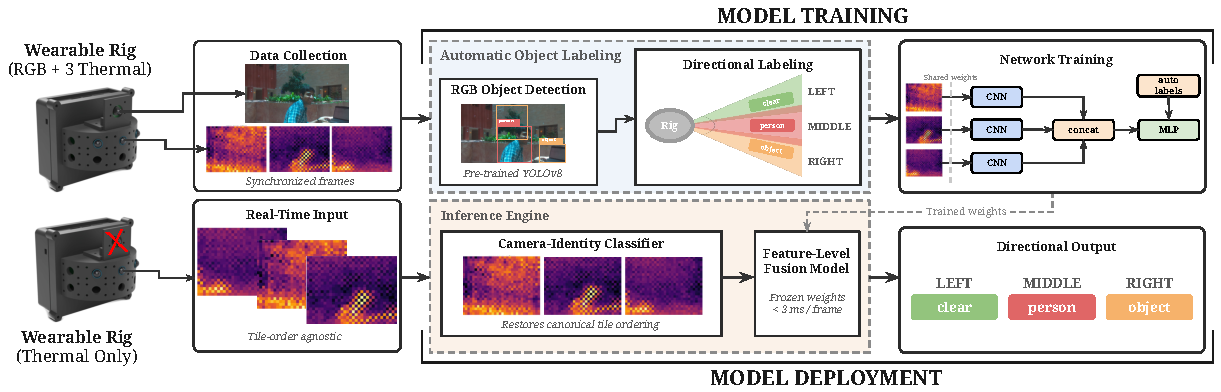
\includegraphics[width=0.9\textwidth]{figs/fig1.pdf}
  \caption{End-to-end pipeline. Top: RGB/YOLOv8 auto-labels supervise the shared-weight CNN backbone with no manual annotation. Bottom: thermal-only tiles, re-sorted by the camera-identity classifier, feed the frozen Feature Fusion model for three-class directional output. Inferno colormap for display only.}
  \label{fig:pipeline}
\end{figure*}



\section{Related Work}
This section reviews the literature most closely related to wearable navigability estimation using privacy-preserving thermal sensing and multi-view perception.
\subsection{Wearable Navigation and Traversability Estimation}
Existing wearable navigation systems estimate traversable space with sensors
that are accurate but hardware-heavy and privacy-invasive. Most rely on RGB
cameras~\cite{11540071}, depth sensors, or LiDAR~\cite{Liu_2021_ICCV} to
detect obstacles and identify safe directions for movement. RGB-based methods
infer navigability from visual
appearance~\cite{muDynamicObstacleAvoidance2024}, whereas depth- and
LiDAR-based systems rely on explicit geometric measurements of the
environment. These sensing requirements increase hardware complexity and raise
privacy concerns for continuous wearable
deployment~\cite{rinta-homiHowLowCan2021}.

\subsection{Privacy-Preserving and Ultra-Low-Resolution Thermal Sensing}

Privacy-preserving thermal sensing has emerged as a promising alternative to RGB-based perception for wearable navigation, enabling continuous environmental sensing while reducing concerns associated with capturing identifiable imagery~\cite{papagianopoulos2023obstacle}. Recent work has demonstrated the feasibility of thermal-based obstacle detection using standard-resolution thermal cameras. In particular, DareDevil~\cite{gaoDeployablePrivacyPreservingThermalBased2025} leverages a paired RGB camera and a pretrained YOLOv8 detector to automatically label thermal frames, eliminating the need for manual annotation while performing thermal-only obstacle detection at inference. However, DareDevil operates on imagery from a single standard-resolution thermal camera ($640\times480$) and formulates the task as binary obstacle detection. It therefore does not investigate directional navigability estimation, multi-camera thermal perception, or the challenges posed by ultra-low-resolution thermal sensing.

% DareDevil~\cite{gaoDeployablePrivacyPreservingThermalBased2025} is the closest
% precedent to our labeling pipeline, auto-labeling thermal frames from a paired
% RGB camera through a pretrained YOLOv8 detector and thereby avoiding manual
% annotation. However, DareDevil collapses all
% object classes into a single binary obstacle label and operates on colorized
% thermal frames from a single standard-resolution thermal camera at inference
% time. It does not address the extreme spatial compression of a
% $32\times24$-pixel array, multi-camera fusion, or robustness to sensor
% placement.

Ultra-low-resolution thermal arrays further improve privacy, cost, and power efficiency, but introduce substantially greater perception challenges due to their extremely limited spatial resolution. Existing work has therefore focused on tasks such as occupancy detection~\cite{rinta-homiHowLowCan2021}, human monitoring~\cite{rezaeiUnobtrusiveHumanActivity2023}, and motion estimation rather than scene understanding or navigability. For example, Mohsen et al.~\cite{mohsenDeepFusionUltraLowResolution2025} combine thermal imagery with gyroscope measurements to compensate for the limited visual information available for odometry.
% while Naser et al.~\cite{naser2022calibration} assume a fixed, calibrated sensor geometry. 
Whether ultra-low-resolution thermal sensing alone can support directional navigability estimation in a wearable multi-camera setting remains largely unexplored.

% tete line of work uses ultra-low-resolution thermal sensors (e.g.,
% $32\times24$ arrays, on the order of \$30 per unit) as a low-power,
% lighting-invariant alternative to RGB and depth sensing. Such sensors are too
% coarse to resolve identifiable facial features, but their reduced spatial
% detail also degrades the features on which downstream perception models rely.
% Prior work compensates for this by fusing thermal imagery with gyroscope
% readings for motion estimation~\cite{mohsenDeepFusionUltraLowResolution2025}.
% Naser~\textit{et al.}~\cite{naser2022calibration} separately showed that most
% low-resolution thermal pipelines still assume a fixed, calibrated sensor
% geometry. In contrast, this work targets discrete navigability classification
% rather than continuous odometry, and removes the reliance on precise geometric
% calibration at inference that these systems retain.

% Removed, not very relevant
% \subsection{Automatic Label Generation}
% Manually annotating walkable regions is expensive and does not scale to
% real-world indoor environments. Kim~\textit{et al.}~\cite{kim2024traversability}
% addressed this for egocentric video with an automated annotation strategy that
% derives traversability labels without manual pixel-level annotation. At larger
% scale, CityWalker~\cite{liuCityWalkerLearningEmbodied2025} trains an embodied
% urban navigation policy on over 2{,}000 hours of in-the-wild web video,
% replacing teleoperated demonstrations with pseudo-labels derived from visual
% odometry. We apply the same philosophy in a cross-modal setting, where
% RGB-derived object detections supervise a thermal-only model solely during
% data collection and the RGB sensor is entirely absent at deployment.

\subsection{Multi-View Sensor Fusion and Placement Robustness}

Multi-view perception systems combine observations from multiple cameras to increase environmental coverage and improve perception quality~\cite{zhuAutonomousRobotNavigation2020,olagokeLiteratureSurveyMultiCamera2020}. Existing systems typically aggregate information from multiple cameras within a unified perception pipeline~\cite{Zheng_2023_WACV}, although the choice of where and how to combine observations varies across applications. In contrast to prior work, this paper investigates how different fusion strategies perform for directional navigability estimation from wearable ultra-low-resolution thermal sensing, while also evaluating their robustness to changes in camera placement.

Wearable multi-camera platforms introduce an additional deployment challenge: the physical arrangement of sensors may change between training and deployment as cameras are repositioned or reattached. Existing multi-camera perception systems are typically designed for fixed camera configurations, an assumption that simplifies geometric reasoning and sensor fusion but is difficult to maintain in wearable platforms~\cite{kuoRedesigningSLAMArbitrary2020}. Consequently, changing the mapping between physical cameras and network input channels can degrade the performance of fusion models that exploit camera-specific spatial relationships. In this work, we evaluate the robustness of representative fusion strategies to camera permutations and investigate lightweight mechanisms for maintaining performance under changing sensor arrangements.

Taken together, the literature reviewed above has not established whether wearable ultra-low-resolution multi-view thermal sensing can reliably support directional navigability estimation under realistic deployment conditions.
% Multi-camera perception systems typically assume a fixed mapping between
% physical sensor position and input channel, an assumption that breaks when
% sensors shift or are reattached in a different order on a wearable rig.
% Pixel-level, decision-level, and feature-level fusion are well studied in the
% sensor fusion literature, but little work examines how these strategies behave
% when the camera-to-slot assignment is perturbed, particularly at the small
% camera counts and extreme resolutions considered here. This also relates to
% cross-resolution knowledge transfer, where a high-resolution signal supervises
% a model on coarser inputs~\cite{qiMultiScaleAlignedDistillation2021}. Our gap
% is larger still, since the supervisory RGB detector and the deployed
% $32\times24$ thermal arrays share no feature space and no geometric alignment
% at inference time. 

%We contribute a direct comparison of three fusion strategies for an ultra-low-resolution, three-camera array, together with an explicit treatment of camera-slot permutation robustness.

\section{Methodology}

This section describes the proposed framework for directional navigability estimation from wearable ultra-low-resolution thermal sensing. We first formulate the prediction task and describe the RGB-based automatic label generation procedure. We then present the evaluated multi-view fusion architectures and the camera-identity correction used to improve robustness to changing sensor arrangements.

\subsection{Problem Formulation}

At each timestep the rig outputs three thermal tiles
$\{x_{\text{L}}, x_{\text{M}}, x_{\text{R}}\}$, one from each active camera,
each $32\times24$. For each direction
$d \in \{\text{left}, \text{middle}, \text{right}\}$ the model predicts
$y_d \in \{\text{clear}, \text{person}, \text{other object}\}$, where clear denotes an unobstructed direction. Separating person from other object is valuable in practice, since a person may yield or move out of the path whereas a static object will not, allowing a navigation aid to respond differently to each. At
inference, the model observes only the thermal tiles:
$f: (x_{\text{L}}, x_{\text{M}}, x_{\text{R}}) \mapsto (y_{\text{L}},
y_{\text{M}}, y_{\text{R}})$. 
Training labels are generated from the paired RGB stream (Section~\ref{sec:labels}), with unlabeled directions masked during optimization.

\subsection{RGB-Based Automatic Label Generation}
\label{sec:labels}

Our automatic labeling procedure builds upon the methodology proposed by DareDevil~\cite{gaoDeployablePrivacyPreservingThermalBased2025}. Unlike in their single-camera formulation, object detections are assigned independently to the three thermal cameras using coarse footprint overlap rather than pixel-accurate RGB-to-thermal alignment. This requires a one-time RGB-to-thermal homography calibration for each of the three thermal cameras, performed once when the rig is built; each homography routes RGB bounding boxes into the corresponding thermal camera's footprint and thereby defines which detections belong to the left, middle, and right directions during training.


% We follow Gao~\textit{et al.}'s
% DareDevil~\cite{gaoDeployablePrivacyPreservingThermalBased2025} in using a
% paired RGB camera and a pretrained detector to auto-label thermal frames
% without manual annotation. The extension here is multi-camera labeling that
% tolerates coarse alignment. Instead of relying on a single pixel-accurate
% RGB-to-thermal correspondence, each detection is routed to a direction by
% bounding-box overlap with a per-camera image footprint (below), so the three
% independent RGB-to-thermal homographies on this rig need only be approximately
% correct.
Each RGB frame is processed by YOLOv8 (You Only Look Once) \cite{yolov8_ultralytics}. Person detections are assigned the label person, while all remaining detections are assigned the label other object. Labels are mapped to thermal directions based on footprint overlap with the corresponding thermal camera. Directions with no overlapping detections are labeled clear. Invalid footprints are masked during training.
y
% Labels are generated from synchronized RGB frames with no manual step. Each
% frame is passed through a pretrained YOLOv8 detector. Its person category
% becomes our \textit{person} label, and every other detected object becomes our
% \textit{other-object} label. To assign a detection to a direction, its bounding
% box is checked for overlap with the image footprint of each thermal camera,
% using RGB-to-thermal homographies fixed once when the rig is built. A direction
% is labeled \textit{person} if a person box overlaps its footprint,
% \textit{other object} if only a non-person box overlaps, and \textit{clear} if
% nothing overlaps. Directions without a valid footprint are masked out. The
% thermal model never sees RGB at inference and is not trained on aligned RGB
% pixels.

\subsection{Multi-View Fusion Architectures}
\begin{figure*}[!t]
  \centering
  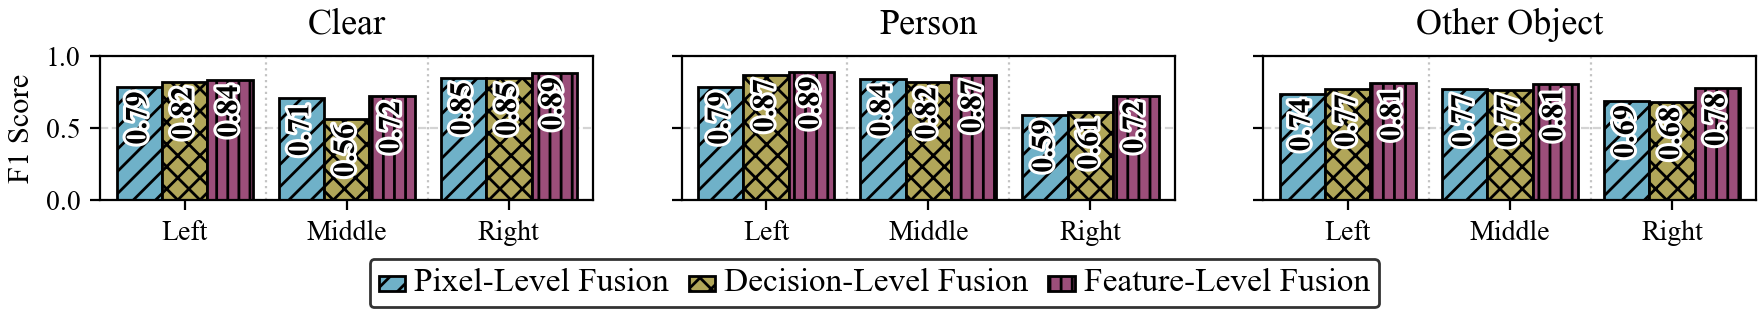
\includegraphics[width=\textwidth]{figs/fig2.png}
  \caption{Per-class $F_1$ by camera direction (left, middle, right) for the
  three fusion strategies: pixel (stitched), decision
  (output fusion), and feature.}
  \label{fig:arch_f1}
\end{figure*}

We evaluate four architectures for estimating per-direction navigability
from three ultra-low-resolution thermal cameras. All models operate directly
on raw single-channel $32\times24$ thermal tiles and produce a three-class
prediction (\textit{clear}, \textit{person}, or \textit{other object}) for
each camera direction. The architectures differ only in how information from
the three views is combined, spanning pixel-level, decision-level, and
feature-level fusion, together with a fourth variant that augments
feature-level fusion with camera-identity correction for placement
robustness. 
Except for the stitched-panorama baseline, all models share the same
convolutional backbone. The backbone consists of a stack of convolutional
blocks whose depth, width multiplier, and activation function are varied
during model selection. Each backbone produces multi-scale feature maps that
are consumed by the downstream fusion and classification modules.
% Except for the stitched-panorama baseline, all models share the
% same convolutional backbone.


% We evaluate four architectures for estimating per-direction navigability from the three active thermal cameras (left, middle, right), each consuming only raw $32\times24$ thermal tiles at inference time and producing a 3-class prediction per camera over $\{\text{clear}, \text{person}, \text{other object}\}$. Tiles are kept as single-channel raw intensity throughout, with no colorization step converting them to pseudo-RGB before the backbone, unlike prior work that colorizes thermal frames for a detector pretrained on natural images. The four span pixel-level, decision-level, and feature-level fusion, plus a fourth variant that adds a learned correction for camera-placement permutations on top of feature-level fusion. All but the stitched-panorama baseline share one configurable convolutional backbone, referred to below as the \textit{shared backbone}. This backbone is a plain stack of convolutional blocks with tunable depth $d \in \{2,\dots,5\}$, a MobileNets-style width multiplier $w$ that scales the channel count of every layer~\cite{howardMobileNetsEfficientConvolutional2017}, and a choice of activation $a \in \{\text{ReLU}, \text{GELU}, \text{LeakyReLU}\}$. It returns the intermediate feature map at every block so that downstream heads can pool over multiple resolutions.

\paragraph{Model 1: Stitched Panorama (pixel-level fusion)}
The three thermal tiles are first warped into a shared panoramic image using
pre-computed thermal-to-thermal homographies, following prior homography-based
thermal alignment approaches~\cite{dahmaniThermalHomographyPhotovoltaic2025,ansarPerformanceEvaluationFeature2024}. A convolutional backbone then predicts
the navigability state of each camera direction from the stitched panorama.
Because fusion occurs before feature extraction, information lost during the
homography warp cannot be recovered by subsequent layers.

% \paragraph{Model 1: Stitched Panorama (pixel-level fusion)} The three raw tiles are warped into a shared panoramic canvas via pre-computed thermal-to-thermal homographies, following prior homography-based approaches to close-range thermal alignment~\cite{dahmaniThermalHomographyPhotovoltaic2025,ansarPerformanceEvaluationFeature2024}. Nearest-neighbor interpolation ensures that warped pixels retain their original raw thermal values rather than being blended with neighbors or with the zero-padded border, yielding a two-channel panorama (raw intensity plus a validity mask). A fixed five-layer backbone is applied independently to each camera's bounding-box crop of the panorama, followed by a shared classification head. Because the panorama is built once, before any learned processing, cross-camera information lost to the homography warp is unavailable to the model. This baseline therefore isolates the cost of fusing at the pixel level.

\paragraph{Model 2: Output Fusion (decision-level fusion)} The shared backbone processes each camera's tile independently, and a per-camera head reduces it to one 3-class logit vector. The three logit vectors are concatenated and passed through a small fusion MLP that refines them jointly. Fusion only ever sees already-classified, low-dimensional logits, so cross-camera interaction is limited to statistical dependencies between directions rather than raw spatial features.
\paragraph{Model 3: Feature Fusion} The same shared-weight backbone runs on each camera's tile, but instead of classifying each camera separately, the feature maps from all three cameras at a given backbone level are concatenated channel-wise and projected back to the original channel count via a learned $1\times1$ convolution, applied at every level. This yields a single fused multi-scale feature pyramid mixing all three cameras at every depth, in contrast to Model 2's late fusion. A shared head then produces the final per-camera logits. We sweep backbone depth, width, activation, and head capacity to select the configuration used as the reference Feature Fusion result throughout this paper. The best-performing configuration uses a backbone depth of 5, a width multiplier of $1.5\times$, GELU activation, a 512-unit classification head, and a dropout rate of $0.1$, and this is the configuration used for Models 3 and Model 4 throughout the rest of the paper.


\paragraph{Model 4: Feature Fusion with camera-identity correction}
Feature Fusion assumes a fixed correspondence between input channels and
physical camera directions, making it sensitive to changes in camera
arrangement. To improve deployment robustness, we introduce a lightweight
camera-identity classifier that predicts the physical direction
(\textit{left}, \textit{middle}, or \textit{right}) of each thermal tile.
Given a possibly shuffled set of tiles, the classifier selects the most likely
camera-to-direction assignment, and the re-ordered tiles are passed to the
unmodified Feature Fusion model. We compare this approach against a blind
condition with no correction and an oracle condition using ground-truth camera
identities.


% \paragraph{Model 4: Feature Fusion with camera-identity correction} Model 3's per-level $1\times1$ projections consume all cameras' features in a fixed slot order, so the projection layer can learn to associate an input slot with a physical direction even though the backbone itself is fully shared and permutation-agnostic. If a sensor is reattached in a different slot at deployment time, this learned positional dependence can degrade predictions. We correct for it with a lightweight auxiliary camera-identity classifier, a compact CNN separate from the shared backbone that takes one raw thermal tile and predicts a 3-way softmax over $\{\text{left}, \text{middle}, \text{right}\}$. The classifier is trained independently using the true camera-to-direction mapping recorded at capture time (its slot-identification accuracy is reported in Section~\ref{sec:results}). At inference, given a possibly shuffled set of tiles, it scores every slot against every direction and selects the assignment that maximizes the total log-probability, enumerated exhaustively over all $3! = 6$ permutations. The re-sorted tiles are then passed to the unmodified Model 3. We compare this against an oracle re-sort using ground-truth identities (an upper bound on achievable robustness) and a blind condition with no correction at all.

All four architectures share the same masked, per-camera, three-class cross-entropy training objective, gated by a per-camera validity mask so that timesteps without a labeled RGB frame do not contribute gradient.

\section{Experimental Setup}


% \subsection{Wearable Thermal Data Collection Platform}
% \label{subsec:platform}

% It consists of three ultra-low-resolution thermal cameras, a synchronized RGB camera, and an embedded acquisition unit. 
% Our wearable platform (Fig.~\ref{fig:pipeline}) is designed around four goals: ultra-low unit cost,
% privacy-preserving sensing, portability, and label-free thermal supervision.
% Low unit cost keeps the platform plausible as an everyday aid. Privacy is
% preserved because the deployed device perceives its surroundings only through
% low-resolution thermal arrays~\cite{tao2018home,tateno2020privacy}.
% Portability ensures that the collected data reflect natural egocentric views
% rather than laboratory conditions. Label-free supervision draws navigability
% labels from a co-recorded reference view instead of hand annotation.

\subsection{Wearable Platform}
\label{subsec:platform}
The wearable platform (Fig.~\ref{fig:pipeline}) consists of an NVIDIA Jetson
Nano, three Melexis MLX90640 thermal cameras arranged in a forward-facing fan,
and a co-mounted Raspberry Pi Camera v2 used only to generate labels. The
thermal cameras provide left, middle, and right views, each a $32\times24$
image at 4\,Hz. The platform is built from commodity components for about
\$471, well below comparable wearable depth-based navigation
systems~\cite{li2025rgbd,bai2019wearable}. Thermal and RGB streams are
timestamped during acquisition and synchronized offline, discarding poorly
aligned samples before training.

% A person registers on
% the camera that faces them, while the other views remain near ambient
% temperature~\cite{newaz2024low,dubail2023privacy,papagianopoulos2023obstacle}.
% Each factory-calibrated camera returns a $32\times24$ array of absolute
% temperatures at 4\,Hz.
% Because the MLX90640 exposes a single fixed
% I\textsuperscript{2}C address, a TCA9548A multiplexer selects one camera
% per transaction.

% \paragraph{RGB supervision camera}
% A Raspberry Pi Camera v2 is rigidly mounted to the top of the thermal housing,
% with its optical axis aligned to the central thermal camera, recording
% $1280\times720$ JPEG frames at 4\,fps. It serves as a training-time supervisory
% instrument only and is not part of the deployed inference pipeline. Its
% high-resolution visible-light view provides the navigability labels for the
% co-recorded thermal frames during training, which avoids hand-annotating the
% low-resolution thermal data~\cite{devaguptapu2019borrow}.

% \paragraph{Packaging and software}
% A USB power bank keeps the unit untethered, and a 3D-printed housing fixes the
% three thermal cameras on a curved front face, with a separate printed case for
% the Jetson. The platform is built from low-cost commodity modules rather than
% the depth cameras used in comparable wearable navigation
% aids~\cite{li2025rgbd,bai2019wearable}, and costs approximately \$471 in
% parts. An on-board service starts and stops all sensors jointly and serves a
% live preview for in-field verification, with each sensor driven by an
% independent capture process so that a single-sensor fault cannot interrupt the
% remaining streams. Every sample is stamped at capture with a
% millisecond-resolution Unix timestamp from the shared system clock, which
% allows frames to be aligned in post-processing without hardware triggering.
% After each recording, the service maps every frame of the slowest stream to
% the temporally nearest frame of each remaining stream, retaining the residual
% offset so that poorly synchronized pairs can be discarded before training.
\subsection{Data Collection}
The dataset\footnote{The thermal frames, labels, and thermal homographies are available at \url{https://huggingface.co/datasets/Faiz3005/TartanThermals_Navigability_Dataset}, and the code at \url{https://github.com/jana-hussien/ershad}. RGB frames are withheld to protect the privacy of recorded individuals.} was collected on
the Carnegie Mellon University in Qatar (CMU-Q) campus and spans a variety of
indoor and outdoor scenes, planned to cover a free, a partially obstructed,
and a fully obstructed path (Table~\ref{tab:environments}); the per-direction
labels themselves come from the detector. A human operator wore
the platform and walked through each environment at a natural pace. Sessions were recorded
both with and without other people present, so that the automatic labeler
encountered a realistic mixture of \textit{clear}, \textit{person}, and
\textit{other-object} events. In total, the platform recorded about 116 minutes of data. The
experiments use 15,868 frames from 12 sessions, split at random into 12,697 for training and 3,171
for validation; a separate session of 988 frames, never used for training
or validation, is held out as the test set for the camera-arrangement
experiments. Fig.~\ref{fig:class_dist} shows the resulting class
distribution.
\begin{figure}[t!]
\begin{center}
\centering
\noindent
$\vcenter{\hbox{%
\begin{minipage}{0.42\linewidth}
\centering
\captionof{table}{Scene types encountered during data collection.}
\label{tab:environments}
\scriptsize
\renewcommand{\arraystretch}{1.0}
\setlength{\tabcolsep}{3pt}
% X column takes whatever width State/People leave, so nothing overlaps in any font
\begin{tabularx}{\linewidth}{@{}>{\raggedright\arraybackslash}Xll@{}}
\toprule
\textbf{Environment} & \textbf{Path} & \textbf{People} \\
\midrule
Open corridors              & Free    & No  \\
Stairwells                  & Free    & No  \\
Covered walkways            & Free    & No  \\
\midrule
Doorways                    & Partial & No  \\
Furniture in~path           & Partial & No  \\
Corridor with bystander     & Partial & Yes \\
\midrule
Crowded~lobbies              & Full    & Yes \\
Waiting~areas                & Full    & Yes \\
Building~entrances           & Full    & Yes \\
\bottomrule
\end{tabularx}
\end{minipage}%
}}$%
\hfill
$\vcenter{\hbox{%
\begin{minipage}{0.53\linewidth}
\centering
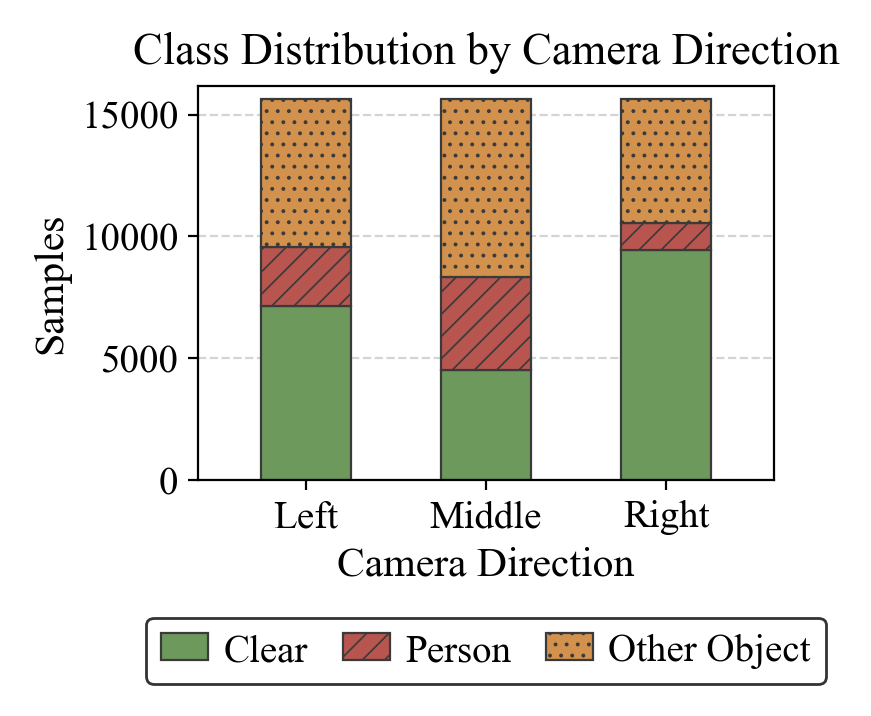
\includegraphics[width=\linewidth]{figs/fig3_new.png}
% 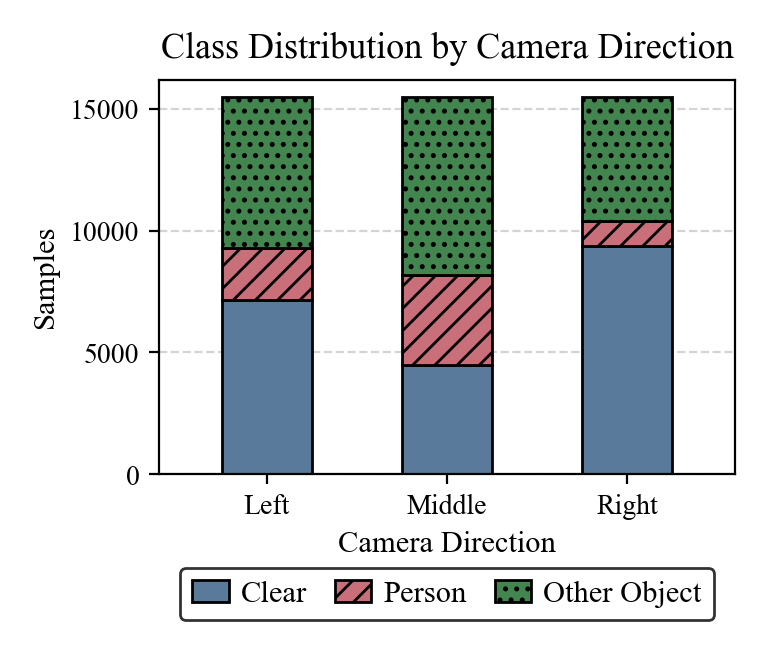
\includegraphics[width=\linewidth]{figs/fig3.png}   % previous version (counts estimated from an image)
\captionof{figure}{Class distribution across camera directions for the combined
training and validation split.}
\label{fig:class_dist}
\end{minipage}%
}}$

\end{center}
\end{figure}
\section{Results}
\label{sec:results}

\subsection{Navigability Estimation Performance}

All four architectures recover navigability well above chance from raw
$32\times24$ tiles, and Feature Fusion leads in every camera direction
(Fig.~\ref{fig:arch_f1}). On validation, Feature Fusion attains overall
per-class $F_1$ of about $0.81$ (\textit{clear}), $0.83$ (\textit{person}),
and $0.80$ (\textit{other object}). The stitched-panorama and output-fusion baselines sit near $0.73$--$0.78$ overall and are weakest on person detection from the right camera.



\subsection{Fusion Strategy Analysis}

Feature-level fusion outperforms both pixel-level stitching and decision-level
output fusion. Concatenating feature maps across cameras at each backbone level
preserves spatial cues that stitching discards in the warp and that output
fusion never observes, since it merges only logits. Feature Fusion requires
additional backbone passes, but at this tile size the accuracy gain justifies
its use in the shuffle experiments below. On a single-sample CPU forward pass,
Model~1, Model~2, and Feature Fusion take 1.36, 0.80, and 2.37\,ms,
respectively, and the camera-identity classifier adds a further 0.21\,ms.
Every configuration remains under 3\,ms, comfortably within budget for
real-time inference on a wearable device.

\subsection{Camera Arrangement Robustness}
\begin{figure}[!t]
    \centering
  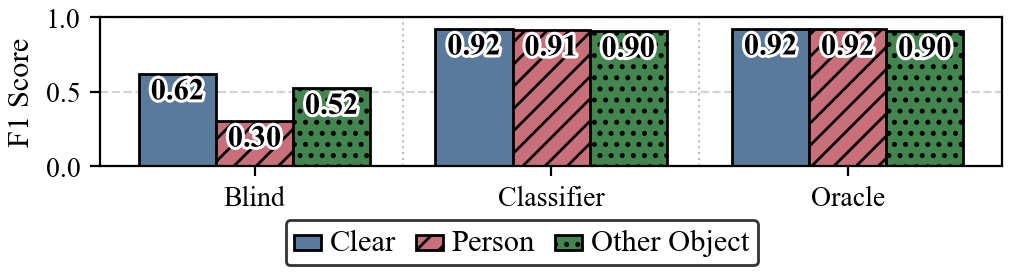
\includegraphics[width=0.9\linewidth]{figs/fig4.png}
  \caption{Overall per-class $F_1$ of Feature Fusion with shuffle correction
  (FF + Shuffle) on the held-out test set (988 frames, not seen during
  training or validation), under blind, classifier, and oracle re-sorting.}
  \label{fig:ff_shuffle}
\end{figure}


Shuffling camera slots collapses uncorrected Feature Fusion, and the
lightweight identity classifier restores it to near-oracle accuracy on the
held-out test set (Fig.~\ref{fig:ff_shuffle}). With no correction (blind),
overall per-class $F_1$ drops to $0.62$ (\textit{clear}), $0.30$
(\textit{person}), and $0.52$ (\textit{other object}), because the fixed-order
projection layers in Model~3 encode slot position. The camera-identity
classifier used to undo this reaches 98.7\% accuracy on the 3-way
slot-identification task on the same 988-frame held-out test set, against a
33.3\% random-guess baseline. Re-sorting the tiles with this classifier before
inference recovers an overall $F_1$ of approximately $0.90$--$0.92$ across all
three classes, matching the ground-truth-identity oracle to within rounding.
The backbone features carry direction information. What breaks under shuffle
is the slot ordering, not the thermal representation itself.
\section{Conclusion}

This paper showed that directional navigability can be learned from three
$32\times24$ thermal cameras using labels generated automatically by an RGB
detector present only at training time. Across four architectures,
feature-level fusion used the limited thermal signal most effectively, and a
lightweight camera-identity classifier made the system robust to camera
rearrangement, restoring near-oracle accuracy at negligible latency cost.
Every model runs in under 3\,ms per frame on CPU, keeping the approach
practical for embedded wearable deployment. Future work includes validating
the identity correction on physically re-mounted sensors and extending the
dataset beyond a single campus.


\FloatBarrier

% \section*{Data Availability}
% The thermal-RGB dataset collected on the wearable platform will be made
% publicly available upon publication.

\bibliographystyle{IEEEtran}
\bibliography{zoteroDetection,ZoteroNav,deviceRefs}

\end{document}
